% !TEX encoding = UTF-8
% !TEX TS-program = pdflatex
% !TEX root = ../tesi.tex
% !TEX spellcheck = it-IT

%**************************************************************
\chapter{Analisi dei Requisiti}
\label{cap:analisi-dei-requisiti}
In questo capitolo sono contenuti i requisiti dell'applicazione che sono stati individuati durante il progetto.\\
Le linee guida per la creazione dell'applicazione sono state fornite dal tutor e sulla base di esse sono stati individuati i requisiti che in seguito sono stati dicussi con il tutor per ottenerne l'approvazione.
%**************************************************************

\section{Applicazione per la modifica dei template}
L'applicazione richiesta per il progetto deve permettere all'utente di visualizzare un insieme di template predefinito, da cui sia possibile selezionare quello desiderato.\\
In seguito alla selezione del template, l'utilizzatore deve poter visualizzare quest'ultimo all'interno di una \textit{view} apposita.\\
In questa fase deve essere fornito all'utente un editor specifico in relazione al template selezionato, che offra la possibilità di visualizzare e modificare i dati forniti di \textit{default} dal template e di vedere all'interno della \textit{view} dedicata il comportamento del template in seguito alla modifica dei dati.\\
L'applicazione deve eseguire all'interno di un browser e deve essere compatibile con i più importanti fra essi (Chrome, Firefox, Opera ed Edge).
\subsection{Visualizzazione lista dei template} \label{subsec:visualizzazione_template}
Questa sezione dell'applicazione è dedicata alla visualizzazione e selezione dei template disponibili.\\
La lista deve essere composta dalle miniature dei template in modo da offrire una prima visione di come viene rappresentato il template.\\
All'utente deve essere permesso di scorrere tutta la lista tramite uno scroll infinito.\\
La lista deve presentare i template per categorie, le seguenti sono quelle individuate durante l'analisi:
\begin{itemize}
	\item template singoli;
	\item template composti;
	\item template singoli contenenti plug-in JQuery;
	\item template composti contenenti plug-in JQuery;
\end{itemize}
I template \textit{singoli} sono dei template la cui costruzione è frutto dell'interpolazione dei dati con un singolo template, mentre quelli \textit{composti} sono template frutto dell'unione di più template.\\
\begin{figure}[htp]
	\centering
	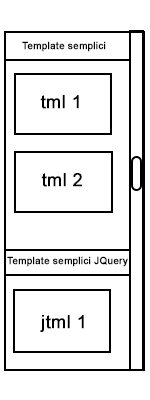
\includegraphics[scale=0.5]{../immagini/mockup_lista}
	\caption{Mockup lista di visualizzazione template.}
\end{figure}

\subsection{Visualizzazione template selezionato}
Questa sezione dell'applicazione è dedicata alla visualizzazione del template selezionato.\\
Il box di visualizzazione non presenta particolari caratteristiche, la sua funzione è quella di mostrare all'utente il template selezionato come verrebbe visualizzato nella pagina html e permettere di osservare i cambiamenti del template in base alla modifica dei dati.
\begin{figure}[htp]
	\centering
	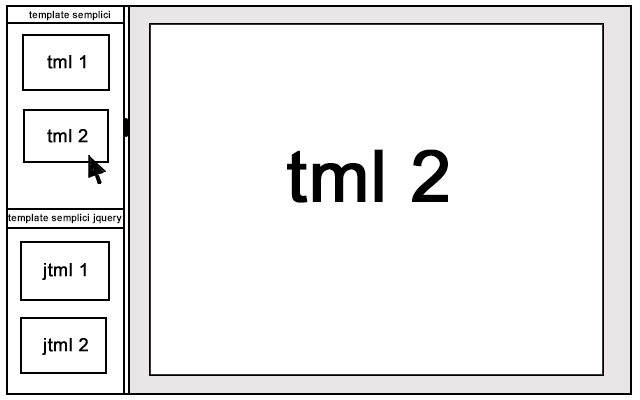
\includegraphics[scale=0.45]{../immagini/mockup_view}
	\caption{Mockup box di visualizzazione template.}
\end{figure}
\subsection{Editor per la modifica del template}
Questa è l'ultima sezione dell'applicazione e si occupa di fornire all'utente gli strumenti per la modifica dei dati relativi al template selezionato.\\
L'utente deve poter visualizzare tutti i dati disponibili per la modifica tramite un interfaccia visuale.\\
Quest'ultima deve fornire all'utente gli strumenti più adeguati per la modifica dei dati in base al loro tipo.\\
Nel caso in cui i template siano composti, l'editor deve visualizzare l'oggetto JSON che rappresenta i dati e dare all'utente la possibilità di modificarne il codice.

%%%%%%%%%%%%%%%%%%%%%%%%%%%%%%%%%%%%%%%%%%%%%%%%%%%%%%%%%%%%%%%%%%%%%%%
%regole per la creazione myminipage
\newenvironment{myminipage}[1]{\minipage{#1} 
	\captionsetup{width=\textwidth, name=Fig., labelfont={it,bf}}
}{\endminipage}
%%%%%%%%%%%%%%%%%%%%%%%%%%%%%%%%%%%%%%%%%%%%%%%%%%%%%%%%%%%%%%%%%%%%%%%
\begin{figure}[htpb] 
	\begin{myminipage}{0.40\textwidth} 
		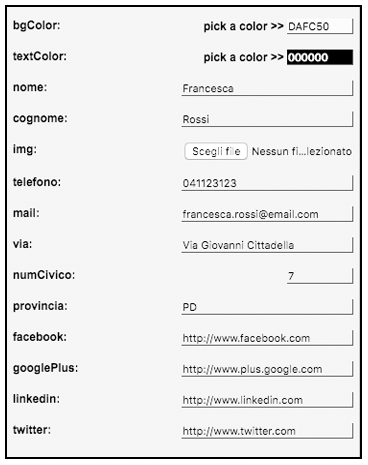
\includegraphics[scale=0.52]{../immagini/mockup_editor1} 
		\caption[Prima figura]{Editor template semplici.}\label{fig:1} 
	\end{myminipage} 
	\hspace{0.1\textwidth} 
	\begin{myminipage}{0.40\textwidth}
		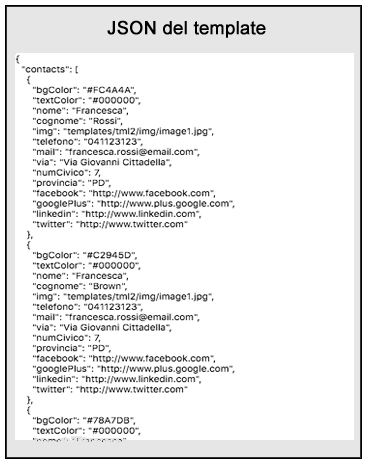
\includegraphics[scale=0.52]{../immagini/mockup_editor2_2}
		\caption[Seconda figura]{Editor template composti.}\label{fig:2} 
	\end{myminipage}  
\end{figure}

\newpage
\section{Requisiti individuati}
%parte presa da giacomo
I requisiti individuati sono frutto dall'analisi ed espansione dei requisiti di base e delle discussioni con il tutor aziendale.\\
Di seguito viene descritto il codice con cui sono stati catalogati:
\begin{center}
	\textit{R[T][I][C]}
\end{center}
dove:
\begin{itemize}
	\item \textbf{T}ipo: specifica la tipologia del requisito e può assumere i seguenti valori:
	\begin{itemize}
		\item \textbf{F} - \textit{funzionale}, cioè che determina una funzionalità dell'applicazione;
		\item \textbf{V} - \textit{vincolo}, che riguarda un vincolo che il prodotto deve rispettare.
	\end{itemize}
	\item \textbf{I}mportanza: specifica l'importanza del requisito e può assumere i seguenti valori:
	\begin{itemize}
		\item \textbf{O} - \textit{obbligatorio}, il requisito corrisponde ad un obbiettivo minimo del piano di stage e deve essere soddisfatto per garantire il funzionamento minimo dell'applicazione;
		\item \textbf{D} - \textit{desiderabile}, il requisito corrisponde ad un obbiettivo massimo del piano di stage e deve essere soddisfatto per garantire il funzionamento dell'applicazione;
		\item \textbf{F} - \textit{facoltativo}, indica che il requisito fornisce del valore aggiunto all'applicazione e non era stato previsto nel piano di stage.
	\end{itemize}
	\item \textbf{C}odice: rappresenta un codice che identifica il requisito all'interno di una gerarchia. Questo codice è definito in modo che il requisito \textit{RTIx.y} sia un requisito che va a definire con un grado maggiore di dettaglio alcuni degli aspetti del requisito \textit{RTIx}.
\end{itemize}

%subsection
%\clearpage
\subsection{Requisiti Funzionali}
\normalsize
\begin{longtable}{|l|m{11cm}|}
\hline
\textbf{Id Requisito} & \textbf{Descrizione}\\
\hline
\endhead
RFO1 & L'utente deve poter visualizzare la lista dei template offerti dall'applicazione \\ \hline
RFO1.1 & L'utente deve poter visualizzare le miniature dei template \\ \hline
RFF1.1.1 & La comparsa delle miniature all'interno della lista deve avvenire in modo animato \\ \hline
RFO1.2 & L'utente deve poter scorrere la lista dei template \\ \hline
RFO1.3 & L'utente deve poter visualizzare la categoria dei template \\ \hline
RFO1.4 & L'utente deve poter selezionare i template \\ \hline
RFD1.4.1 & La selezione del template deve avvenire in modo animato \\ \hline
RFO2 & L'utente deve visualizzare il template selezionato in un apposito view-box \\ \hline
RFF2.1 & La comparsa del template nel view-box deve avvenire in modo animato \\ \hline
RFD2.2 & Se il template contiene plug-in JQuery l'utente deve poter visualizzare l'esecuzione del plug-in \\ \hline
RFO2.3 & L'utente deve visualizzare nel view-box l'effetto delle modifiche appotrate al template \\ \hline
RFO2.3.1 & L'utente deve poter visualizzare l'effetto sul template delle modifiche ai dati di tipo colore \\ \hline
RFO2.3.2 & L'utente deve poter visualizzare l'effetto sul template delle modifiche ai dati di tipo numero \\ \hline
RFO2.3.3 & L'utente deve poter visualizzare l'effetto sul template delle modifiche ai dati di tipo booleano \\ \hline
RFO2.3.4 & L'utente deve poter visualizzare l'effetto sul template delle modifiche ai dati di tipo immagine \\ \hline
RFO2.3.5 & L'utente deve poter visualizzare l'effetto sul template delle modifiche ai dati di tipo url \\ \hline
RFO2.3.6 & L'utente deve poter visualizzare l'effetto sul template delle modifiche ai dati di tipo mail\\ \hline
RFO2.3.7 & L'utente deve poter visualizzare l'effetto sul template delle modifiche ai dati di tipo stringa breve\\ \hline
RFO2.3.8 & L'utente deve poter visualizzare l'effetto sul template delle modifiche ai dati di tipo testo \\ \hline
RFO2.3.9 & L'utente deve poter visualizzare l'effetto sul template delle modifiche ai dati di tipo JSON \\ \hline
RFO3 & L'utente deve poter visualizzare i dati di default forniti dal template selezionato \\ \hline
RFO3.1 & L'utente deve poter visualizzare i dati di tipo colore \\ \hline
RFO3.2 & L'utente deve poter visualizzare i dati di tipo numero \\ \hline
RFO3.3 & L'utente deve poter visualizzare i dati di tipo booleano \\ \hline
RFO3.4 & L'utente deve poter visualizzare i dati di tipo immagine \\ \hline
RFO3.5 & L'utente deve poter visualizzare i dati di tipo url \\ \hline
RFO3.6 & L'utente deve poter visualizzare i dati di tipo mail \\ \hline
RFO3.7 & L'utente deve poter visualizzare i dati di tipo stringa breve \\ \hline
RFO3.8 & L'utente deve poter visualizzare i dati di tipo testo \\ \hline
RFO3.9 & L'utente deve poter visualizzare i dati in formato JSON \\ \hline
RFO4 & L'utente deve poter modificare i dati di default forniti dal template selezionato \\ \hline
RFO4.1 & L'utente deve poter modificare i dati di tipo colore \\ \hline
RFD4.1.1 & L'utente deve poter visualizzare il color-picker \\ \hline
RFF4.1.1.1 & La comparsa del color-picker deve avvenire in modo animato \\ \hline
RFF4.1.1.2 & La scomparsa del color-picker deve avvenire in modo animato \\ \hline
RFD4.1.2 & L'utente deve poter selezionare il colore nel color-picker \\ \hline
RFO4.2 & L'utente deve poter modificare i dati di tipo numero \\ \hline
RFO4.3 & L'utente deve poter modificare i dati di tipo booleano \\ \hline
RFO4.4 & L'utente deve poter modificare i dati di tipo immagine \\ \hline
RFD4.4.1 & L'utente deve poter caricare un'immagine da filesystem \\ \hline
RFO4.5 & L'utente deve poter modificare i dati di tipo url \\ \hline
RFO4.6 & L'utente deve poter modificare i dati di tipo mail \\ \hline
RFO4.7 & L'utente deve poter modificare i dati di tipo stringa breve \\ \hline
RFO4.8 & L'utente deve poter modificare i dati di tipo testo \\ \hline
RFO4.9 & L'utente deve poter modificare i dati dell'oggetto in formato JSON \\ \hline
RFD5 & L'utente deve poter visualizzare un messaggio di errore nel caso in cui l'inserimento dei dati avvenga in maniera non corretta \\ \hline

\caption[Requisiti Funzionali]{Requisiti Funzionali}
\label{tabella:req0}
\end{longtable}
\clearpage
\subsection{Requisiti di Vincolo}
\normalsize
\begin{longtable}{|l|m{11cm}|}
\hline
\textbf{Id Requisito} & \textbf{Descrizione} \\
\hline
\endhead
RVO1 & L'applicazione deve utilizzare HTML5 \\ \hline
RVO2 & L'applicazione deve utilizzare CSS3 \\ \hline
RVO3 & L'applicazione deve utilizzare JavaScript \\ \hline
RVO4 & L'applicazione deve utilizzare Ractive.js \\ \hline
RVO5 & L'applicazione deve funzionare su \textit{Google Chrome} versione 52.0 o superiore \\ \hline
RVO6 & L'applicazione deve funzionare su \textit{Firefox} versione 46.0 o superiore \\ \hline
RVD7 & L'applicazione deve funzionare su \textit{Safari} versione 9.0 o superiore \\ \hline
RVD8 & L'applicazione deve funzionare su \textit{Edge} versione 37.0 o superiore \\ \hline
RVD9 & L'applicazione deve funzionare su \textit{Opera} versione 37.0 o superiore \\ \hline
RVF10 & L'applicazione deve funzionare su \textit{Internet Explorer} versione 11.0 o superiore \\ \hline
\caption[Requisiti di Vincolo]{Requisiti di Vincolo}
\label{tabella:req1}
\end{longtable}


\section{Riepilogo requisiti}
I requisiti individuati sono in totale 56 e vengono ripartiti tra le varie tipologie secondo quanto riportato nelle seguenti tabelle.
\\ \\ \\
\begin{minipage}{\textwidth}
	\begin{minipage}[b]{0.49\textwidth}
		\centering
		\begin{tabular}{|l|c|} \hline
			\textbf{Importanza} & \textbf{\#} \\ \hline
			Obbligatori & 42 \\ \hline
			Desiderabili & 9 \\ \hline
			Facoltativi & 5 \\ \hline
			Totale & 56 \\ \hline
		\end{tabular}
		\captionof{table}{Numero di requisiti per importanza}
	\end{minipage}
	\hfill
	\begin{minipage}[b]{0.49\textwidth}
		\centering
		\begin{tabular}{|l|c|} \hline
			\textbf{Tipologia} & \textbf{\#} \\ \hline
			Funzionali & 46 \\ \hline
			Vincolo & 10 \\ \hline
			Totale & 56 \\ \hline
		\end{tabular}
		\captionof{table}{Numero di requisiti per tipologia}
	\end{minipage}
\end{minipage}
\\ \\ \\

\begin{minipage}{\textwidth}
	\begin{minipage}[b]{0.49\textwidth}
		\centering
		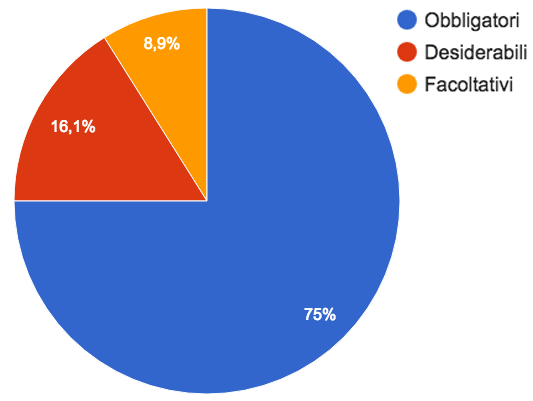
\includegraphics[scale=0.35]{../immagini/chart_requisiti_importanza}
		\captionof{figure}{Requisiti per importanza}
	\end{minipage}
	\hfill
	\begin{minipage}[b]{0.49\textwidth}
		\centering
		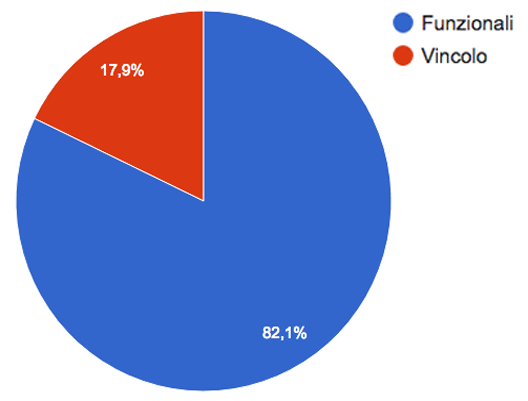
\includegraphics[scale=0.35]{../immagini/chart_requisiti_tipo}
		\captionof{figure}{Requisiti per tipologia}
	\end{minipage}
\end{minipage}
